\documentclass{article}

% if you need to pass options to natbib, use, e.g.:
% \PassOptionsToPackage{numbers, compress}{natbib}
% before loading nips_2017
%
% to avoid loading the natbib package, add option nonatbib:
% \usepackage[nonatbib]{nips_2017}

\usepackage[final]{nips_2017}

% to compile a camera-ready version, add the [final] option, e.g.:
% \usepackage[final]{nips_2017}

\usepackage[utf8]{inputenc} % allow utf-8 input
\usepackage[T1]{fontenc}    % use 8-bit T1 fonts
\usepackage{hyperref}       % hyperlinks
\usepackage{url}            % simple URL typesetting
\usepackage{booktabs}       % professional-quality tables
\usepackage{subfig}         % block figures
\usepackage{amsfonts}       % blackboard math symbols
\usepackage{nicefrac}       % compact symbols for 1/2, etc.
\usepackage{microtype}      % microtypography
\usepackage[pdftex]{graphicx}

\title{A Comparison of Activation Functions in Densely Connected Neural Nets}

% The \author macro works with any number of authors. There are two
% commands used to separate the names and addresses of multiple
% authors: \And and \AND.
%
% Using \And between authors leaves it to LaTeX to determine where to
% break the lines. Using \AND forces a line break at that point. So,
% if LaTeX puts 3 of 4 authors names on the first line, and the last
% on the second line, try using \AND instead of \And before the third
% author name.

\author{
  Zachary Owen
  \thanks{ zaowen.github.io } \\
  Department of Math and Computer Science\\
  South Dakota School of Mines and Technology\\ 
  Rapid City, SD 57701 \\
  \texttt{zacharyowen@acm.} \\
}

\begin{document}
% \nipsfinalcopy is no longer used

\maketitle

\begin{abstract}
        insert abstract here
\end{abstract}

\section{Introduction}

Convolutional neural networks ( CNN's ) are a standard model for identifying structures in visual mediums.
In a world where self driving cars and manufacturing automation are wanting for greater and greater capabilities, CNN's have become deeper and deeper.
The increase in layers is necessary due to the newer and more extensive demands for identifying more varied and complex inputs.
Recent networks containing Convolutions like Highway Networks and Residual Networks have had in excess of 100 layers.
This sort of deep layering causes problems when it comes to backwards and forwards propagation as effects early or late in the network may not properly propagate through or back when it would be necessary.

Earlier this year Huang proposed a new architecture of CNN to simply solve this problem called the Densely Connected Convolutional Network.
This network functions on a stacking of convolutions with the output from every previous convolution as an additional input see Figure \ref{fig:DenseBlock}.

This network is not the focus of this paper however, instead it simply forms a convenient basis for the testing of activators in CNN's.
Since every dense block has identical structure and activators ( ignoring the classification layer ), the activators can be easily swapped out for another activator.
In this paper, we will examine the difference between the different activators supplied by the \textbf{keras python api}.

\subsection{Background}
Densely Connected Convolutional Networks are a very new concept, the paper describing which only being published in January 2018.
{\it DenseNet's} as they are called, are in no small way a response to the recent rise of ResNets ( or Residual Networks). Part of the structure of a Residual network is the passing of the feature map of the previous convolution into the some function with the current convolution.
This has several defects which DenseNets sidestep:
\begin{itemize}
        \item Parameter inefficiency: due to the fact that ResNets require many levels of convolution and every layer requires its own weights. This alone wouldn't be a problem if it weren't for
        \item Lack of Parameter effect It has been shown that in some variations of ResNets, most layers contribute very little information overall and oftentimes can be removed.
        \item Layer inefficiency: Due to the combining of previous layers the models become even larger.
\end{itemize}
DenseNet's instead explicitly save the previous state of the network so it can be fed into the later layers.
This has the additional benefit of not requiring as the convolutional be as wide.

Finally, Backwards propagation on DenseNets does not suffer diminishing returns as it propagates to the start of the network.
Since every layer has direct access to the previous layers loss propagates much more easily.
\begin{figure}
        \centering
        \includegraphics[width=0.3\linewidth]{figures/dense_block}
        \caption{A 5-layer dense block. Each layer takes all preceding convolutions as input.}
        \label{fig:DenseBlock}
\end{figure}

\subsection{Methods}
The original paper uses the ReLU activator and tests very well on several different common sets including CIFAR10, CIFAR100, SVHN and ILSVRC 2012.
A partial goal of this paper is to show if an activator other than the proposed ReLU can perform better than the one in the original paper.
We will be using both Stochastic Gradient Descent (SGD) and Adam as an optimizer. SGD is used in the original paper, but experimentally, Adam performs slightly quicker on the hardware available.
Additionally fewer dense blocks are used due to lack of memory.

We expect both of these caveats to affect the performance of the overall network.

We decided to test four different common activators, Rectified Linear Unit (ReLU), Sigmoid, SoftMax and Hyperbolic Tangent.
These activators were chosen by their popular historical use, popular current use and because we thought SoftMax would be funny.

\section{ Initial Testing}

While doing short runs of testing to get a baseline of how well the networks are performing.
Each was ran for 30 epochs with the Adam optimizer.
Adam was chosen instead of the SGD described in the original paper because training optimized far quicker than with SGD see, Figure \ref{fig:ReLUSGD} for an example of this.
This slowness is why Adam was eventually chosen as the optimizer of choice for this experiment.
\begin{figure}
        \centering
        \subfloat[ReLU]{
        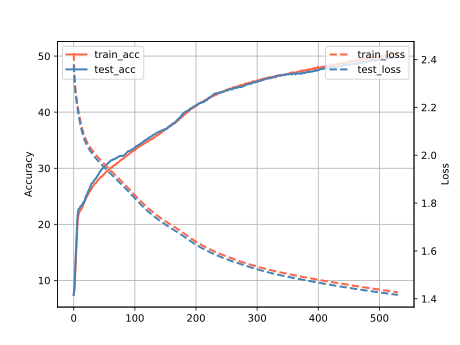
\includegraphics[width=0.5\linewidth]{figures/Adam30/relu_cifar10.pdf}
        }
        \subfloat[Sigmoid]{
        \includegraphics[width=0.5\linewidth]{figures/Adam30/sigmoid_cifar10.pdf}
        }
        \newline
        \subfloat[SoftMax]{
        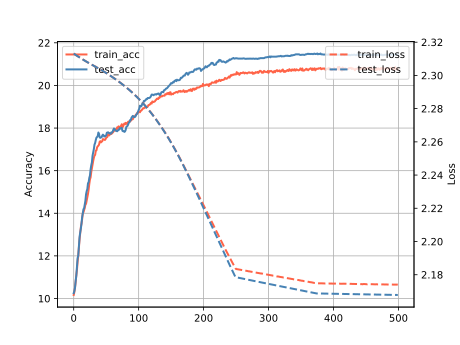
\includegraphics[width=0.5\linewidth]{figures/Adam30/softmax_cifar10.pdf}
        }
        \subfloat[Tanh]{
        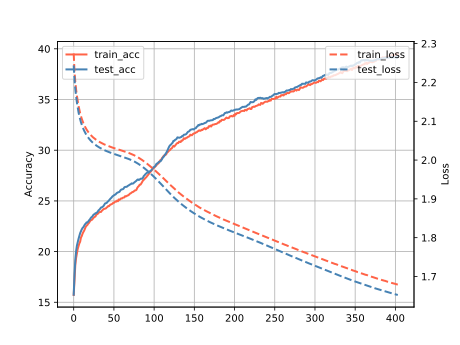
\includegraphics[width=0.5\linewidth]{figures/Adam30/tanh_cifar10.pdf}
        }
        \caption{Densenet with Diffrent Activators. Adam Optimizer, 30 iterations}
        \label{fig:Adam30}
\end{figure}

As you can see from Figure \ref{fig:Adam30}, while all all four activator approach their first local minimum at very similar rates.
The major and important difference is the value which they approach.
ReLU performs the best able to obtain test accuracy that puts it the network above a coin flip.
SoftMax and Hyperbolic Tangent wallow in the low 40\%'s like a chilly spring morning.
Sigmoid on the other hand is just barely able to exceed correct classification on one third of the test set.

While it seems like Sigmoid is least effective, I would like to draw your attention to a fact that will become important later.
In Figure \ref{fig:Adam30}b), while the overall accuracy is low, the delta between the testing and training accuracy is also very small.
This is also true for ReLU and SoftMax, conversely, Hyperbolic Tangents accuracies differ by almost 5\% between training and test, and nearly 10\% overall.
So even though Hyperbolic Tangent achieves the second greatest accuracy it shows symptoms of drastic over-training.
This problem was not discovered at this point in the experiment, however, and instead was not attended to until later when it will be come much more apparent.

\section{Classical Training}

Since the original paper specified SGD as the training method of choice
\begin{figure}
        \centering
        \includegraphics[width=0.8\linewidth]{figures/SGD3k/relu.pdf}
        \caption{Densenet with ReLUconv. SGD Optimizer, 300 iterations}
        \label{fig:ReLUSGD}
\end{figure}

\begin{figure}
        \centering
        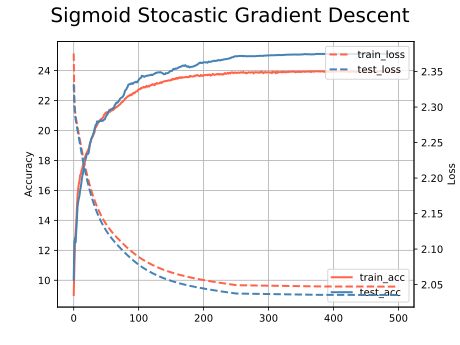
\includegraphics[width=0.8\linewidth]{figures/SGD3k/sigmoid.pdf}
        \caption{Densenet with Sigmoidconv. SGD Optimizer, 300 iterations}
\end{figure}

\begin{figure}
        \centering
        \includegraphics[width=0.8\linewidth]{figures/SGD3k/softmax.pdf}
        \caption{Densenet with Softmaxconv. SGD Optimizer, 300 iterations}
\end{figure}

\begin{figure}
        \centering
        \includegraphics[width=0.8\linewidth]{figures/SGD3k/tanh.pdf}
        \caption{Densenet with Tanhconv. SGD Optimizer, 300 iterations}
\end{figure}

\begin{figure}
        \centering
        \includegraphics[width=0.8\linewidth]{figures/Adam500/relu.pdf}
        \caption{Densenet with ReLUconv. Adam Optimizer, 500 iterations}
\end{figure}

\begin{figure}
        \centering
        \includegraphics[width=0.8\linewidth]{figures/Adam500/tanh.pdf}
        \caption{Densenet with Tanhconv. Adam Optimizer, 500 iterations}
\end{figure}

\begin{figure}
        \centering
        \includegraphics[width=0.8\linewidth]{figures/RELU5kcifar10.pdf}
        \caption{Densenet with ReLUconv. Adam Optimizer, 5000 iterations}
\end{figure}

\begin{figure}
        \centering
        \includegraphics[width=0.8\linewidth]{figures/10kAdam.pdf}
        \caption{Densenet with ReLUconv. Adam Optimizer, 10000 iterations}
\end{figure}


\end{document}
